\documentclass[12pt,a4paper]{article}
% \usepackage[english]{babel}
% \usepackage[utf8x]{inputenc}

\usepackage{graphicx} % Required for inserting images.
\usepackage[margin=25mm]{geometry}
\parskip 4.2pt  % Sets spacing between paragraphs.
% \renewcommand{\baselinestretch}{1.5}  % Uncomment for 1.5 spacing between lines.
\parindent 8.4pt  % Sets leading space for paragraphs.
\usepackage[font=sf]{caption} % Changes font of captions.
\usepackage{subcaption} 
\usepackage{caption}
\usepackage{amsmath}
\usepackage{amsfonts}
\usepackage{amssymb}
\usepackage{siunitx}
\usepackage{verbatim}
\usepackage{gensymb}
\usepackage{placeins}
\usepackage{listings}
\usepackage{xcolor}
\usepackage{float}
\usepackage{graphicx}
\usepackage{todonotes}
\setlength{\marginparwidth}{2cm}  % or even 3cm
\usepackage{subcaption}

\usepackage{hyperref} % Required for inserting clickable links.
\usepackage{natbib} % Required for APA-style citations.


\title{MGAIA Assignment 2: Battlesnakes}
\author{
    Eirini Chrysovergi - s3972453 \\
    Benard Wanyande - s4581733 \\
    }

\begin{document}
\maketitle

\tableofcontents

\section{Introduction}\label{sec:intro}

\section{Methods}\label{sec:methods}

\subsection{Game Rules}
Aim of the game is for the snake to stay alive as long as possible. The rules are:
\begin{enumerate}
    \item Every turn costs 1 HP. 
    \item An agent has 100 ms to perform that turn, otherwise resulting in a timeout. 
    \item The maximum turn limit is 300. 
    \item Starting snake length is 3.
    \item Each time a snake eats a pellet its length is increased by one tile, and its health restores to 100.
    \item There are at minimum 2 food pellets on the board at any given turn, with more spawning constantly.
    \item Moving out of bounds results in elimination.
    \item On head to head collisions between snakes, the larger sized snake survives and the other gets eliminated.
    \item On head to body collisions between snakes the colliding snake gets eliminated. 
    \item Self collisions result in elimination.
    \item Hazard pits appear from turn 26 and stack up every 25 turns, with 4 stacks in total. When fully stacked, it stays that way for 75 turns before fully draining. The first stack causes 14 points of damage to the snake, plus 1 point damage taken per turn. As stacks pile up, damage also piles piles by multiples of 14. Hazards only incur damage to the snake in a head on collision.
    \item A final score is calculated by giving 80\% weightage to snake survival and 20\% weightage to its length.
\end{enumerate}

\subsection{Heuristic Agent}\label{sec:heur-agent}
For the heuristic agent we prioritize immediate survival before pursuing long-term objectives such as size growth. In each state, we evaluate every possible move is against a set of hard constrains (for immediate survival) and soft constrains (where we score the moves based on the long-term survival of the snakes). Our agent operates in a non-deterministic environment as we cannot predict opponent movements, however, we can improve performance by assuming a partial adversarial environment where future moves that will occupied by opponents are considered high risk actions. We simplify the overall state space by treating the board as a grid of discrete hazards and rewards, which we employ a Manhattan distance metric to evaluate the proximity. 

The final decision is given after three stages: filtering, evaluation and selection. In the filtering phase, we eliminate all immediate moves that lead to death, set by the rules of the game. This includes moves of self collision, backwards, or out of bounds movements. To avoid head yo body collisions we assume that the snake opponents bodies are stationary which is not far from the truth as at any movement only the snake's head and tail are the ones that are actually changing. On the other hand, for head to head collisions we followed a more dynamic approach for which any shared adjacent cells between two snakes will be considered as a terminal hazard if an opponent is larger or equal in size. This way, we avoid as much as possible collisions that will result in elimination of our snake agent. 

Once filtering is done, we evaluate the state using a two heuristic component metrics: spatial availability and food proximity. We determine the first through a Breadth First Search (BFS) algorithm, which calculates the reachable flood fill area from a potential next position. We employed this measure, to avoid our snakes from restricting in closed spaces, where our snakes will be eliminated from dead ends. Simultaneously, we evaluate the proximity to the food to prioritize length growth if the HP falls bellow a threshold. We attempted to implement two approaches for that part in order to compare their performances. In the first case, which we name Friendly mode, we only prioritize the length at a starvation state. More precisely, the snake starts to seek for food if the HP drops bellow 40 and, since we want to avoid starvation, it targets food at nearest positions. At the second case, we seek for food at higher HP, with a threshold of 60 and for that reason the food we seek is furthest away from opponents but still reachable. In both cases, whenever we satisfy the HP condition we select moves that prioritize the spatial space. Our final selected move is a random choice of our best moves at a current state.

\subsection{MCTS Agent}
At the start of a run of the MCTS algorithm, the tree consists of a single node representing the current state of the game. The algorithm then iteratively builds a search tree by adding and evaluating new nodes representing game states. This process can be interrupted at any time, rendering MCTS an anytime algorithm. MCTS requires only two pieces of information to operate: the game rules that would, in turn, yield the available moves in the game and the terminal state evaluation—whether that is win, a loss, a draw, or a game score. The vanilla version of MCTS does not require a heuristic function, which is, in turn, a key advantage over Minimax. The core loop of the MCTS algorithm can be divided into four steps: Selection, Expansion (the first two steps are also known as tree policy), Simulation and Backpropagation.

Selection: In this phase, it is decided which node should be expanded. The process starts at the root of the tree, and continues until a node is selected which has unexpanded children. Every time a node (action) is to be selected within the existing tree a child node j is selected to maximise the UCB1 formula:
\begin{equation}
    UCB1 = \bar{X_j} + 2 C_p \sqrt{\frac{2 \ln{n}}{n_j}}
\end{equation}

where $\bar{X_j}$ is the average reward of all nodes beneath this node, $C_p$ is an exploration constant (often set to $1/\sqrt{2}$), n is the number of times the parent node has been visited, and $n_j$ is the number of times the child node j has been visited.

Expansion: When a node is selected that has unexpanded children—i.e., that represents a state from which actions can be taken that have not been attempted yet—one of these children is chosen for expansion, meaning that a simulation is done starting in that state. Selecting which child to expand is often done at random.

Simulation (Default Policy): After a node is expanded, a simulation (or rollout) is done starting from the non-terminal node that was just expanded until the end of game to produce a value estimate. Usually, this is performed by taking random actions until a termination state is reached, i.e., until the game is either won or lost. The state at the end of the game is used as the reward ($\Delta$) for this simulation, and propagated up the search tree. Since in the game environment a snake can survive many turns, the reward function need to reflect the winning score set by the game rules. Thus, we utilize a 80/20 split between survival and length ensuring that even when a path results in death, it will still reward the one that survived the longest and grew the most. In addition, since snakes can survive many turns, instead of simulating until a terminal state is reached, we evaluate states until a rollout depth is reached.

Backpropagation: The reward is propagated back up the path to the root, updating the statistics (visit counts and total rewards) of all the parent nodes.

In our implementation, we assume that the opponents are stationary in order to decrease the branching factor from $4^4$ to just 4. In the standard MCTS every snake would move simultaneously increasing dramatically the computationally time for propagating the tree. Since our decision need to be made in less than 100 ms, this stationary opponent assumption was necessary for the performance of our algorithm. While with this assumption we ignore the behavior of other snakes, it may not be an issue as for each state we reach significantly greater depths. This is often called a paranoid search in games for which we assume that all the other opponents act as collectively as one. This approach selects the moves of our snakes in a conservative manner influencing positively the survival of our snakes. 


Lastly, apart from the vanilla MCTS which uses a random rollout, we guided our simulation steps using our heuristic agent (see Section \ref{sec:heur-agent}) to improve our performance. 

\subsubsection{Hyper-parameter exploration}\label{sec:hyperparameter-exploration}

To maximize the performance of our MCTS agent, we implemented a tournament framework for hyper-parameter exploration. In principal, in order our search to be effective we need to balance the exploration and exploitation governed by $C_p$. In addition, the rollout depth needs to be explored to quantify the quality of our state evaluation versus the actual agent's performance. 

The evaluation of the performance is based on a tournament of 4 snakes, one of which is an MCTS agent with varying hyper-parameter value (either $C_p$ or rollout depth depending on the test) against three similar type heuristic agents that represent a baseline \footnote{Tests were made between 4 MCTS agents, each with a varying hyper-parameter values. The results showed a very noisy performance, possibly because we compare agents of similar performance. Thus, in order to infer best fit values for the hyper-parameter under examination, we ended up using 3 heuristic agents to act as a baseline.}. 

For the evaluation of the performance of the agents we record three important measures: the average turns per hyper-parameter increment, the win rate as well as the TrueSkill rating. This is a conservative estimate of the agent's power level ($\mu-3\sigma$) ensuring that high rating reflects consistent performance. 

For testing the exploration constant we used a uniform range of values of 0.1 to 10.0. In a similar fashion, the rollout depth was varied from 20 to 1000 steps. We present the tournament results after 1000 games as a function of $C_p$ and rollout depth in Figure \ref{fig:hyperparameter exploration}. 

The results indicate that the average turns our MCTS agents survived ranges between 150 to 200 turns, although the dispersion is high, with an error dispersion of 250 in both $Cp$ and rollout depth plots. Given that the true skill rating is a more accurate measure of the performance of our agents we can see that there are two maximums at $C_p=0.1$ and 7.9. Given the performance of the adjacent $C_p$ values at those maximum, we conclude that the value of 7.9 should give us the better performance, although qualitatively the influence of $C_p$ is not a very major with a absolute dispersion of $\sim5$ in the $C_p$ plane. In a similar manner, for the rollout depth we identify that there is one global maximum in the true skill rating plot at 120 turns.





\begin{figure}[h]
    \centering
    
    \begin{subfigure}{0.49\textwidth}
        \centering
        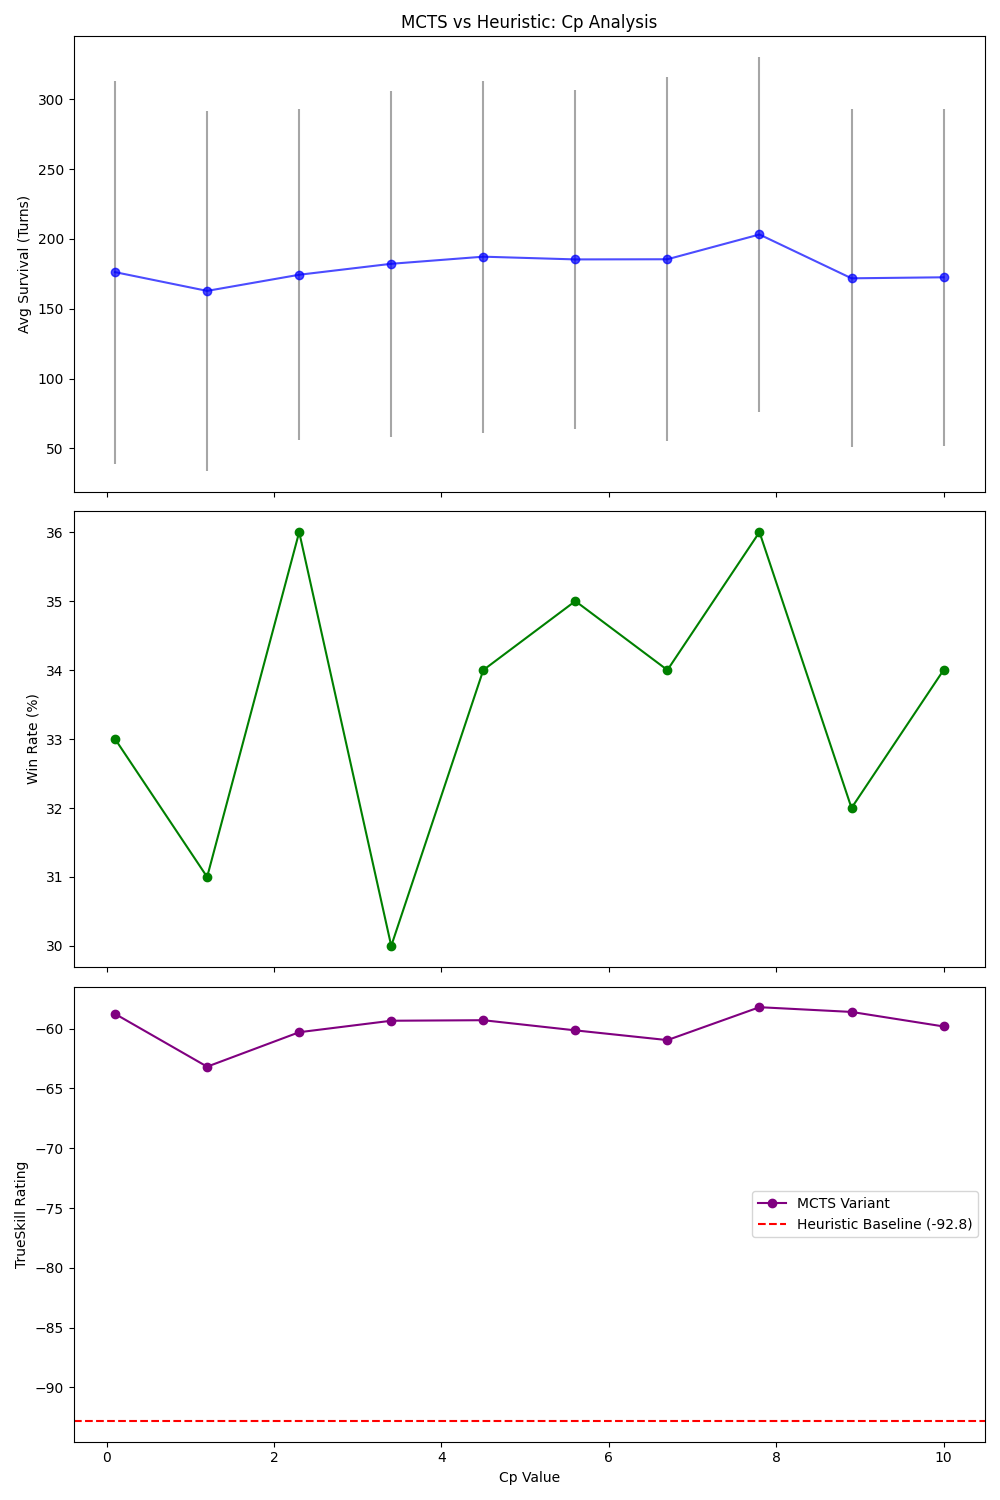
\includegraphics[width=\linewidth]{Figures/Cp_metrics_plot_1000_games.png}
        \caption{Effect of the exploration constant $C_p$ within the range 0 to 10. The rollout depth was fixed to 80.  }
        \label{fig:Cp}
    \end{subfigure}
    \hfill
    \begin{subfigure}{0.49\textwidth}
        \centering
        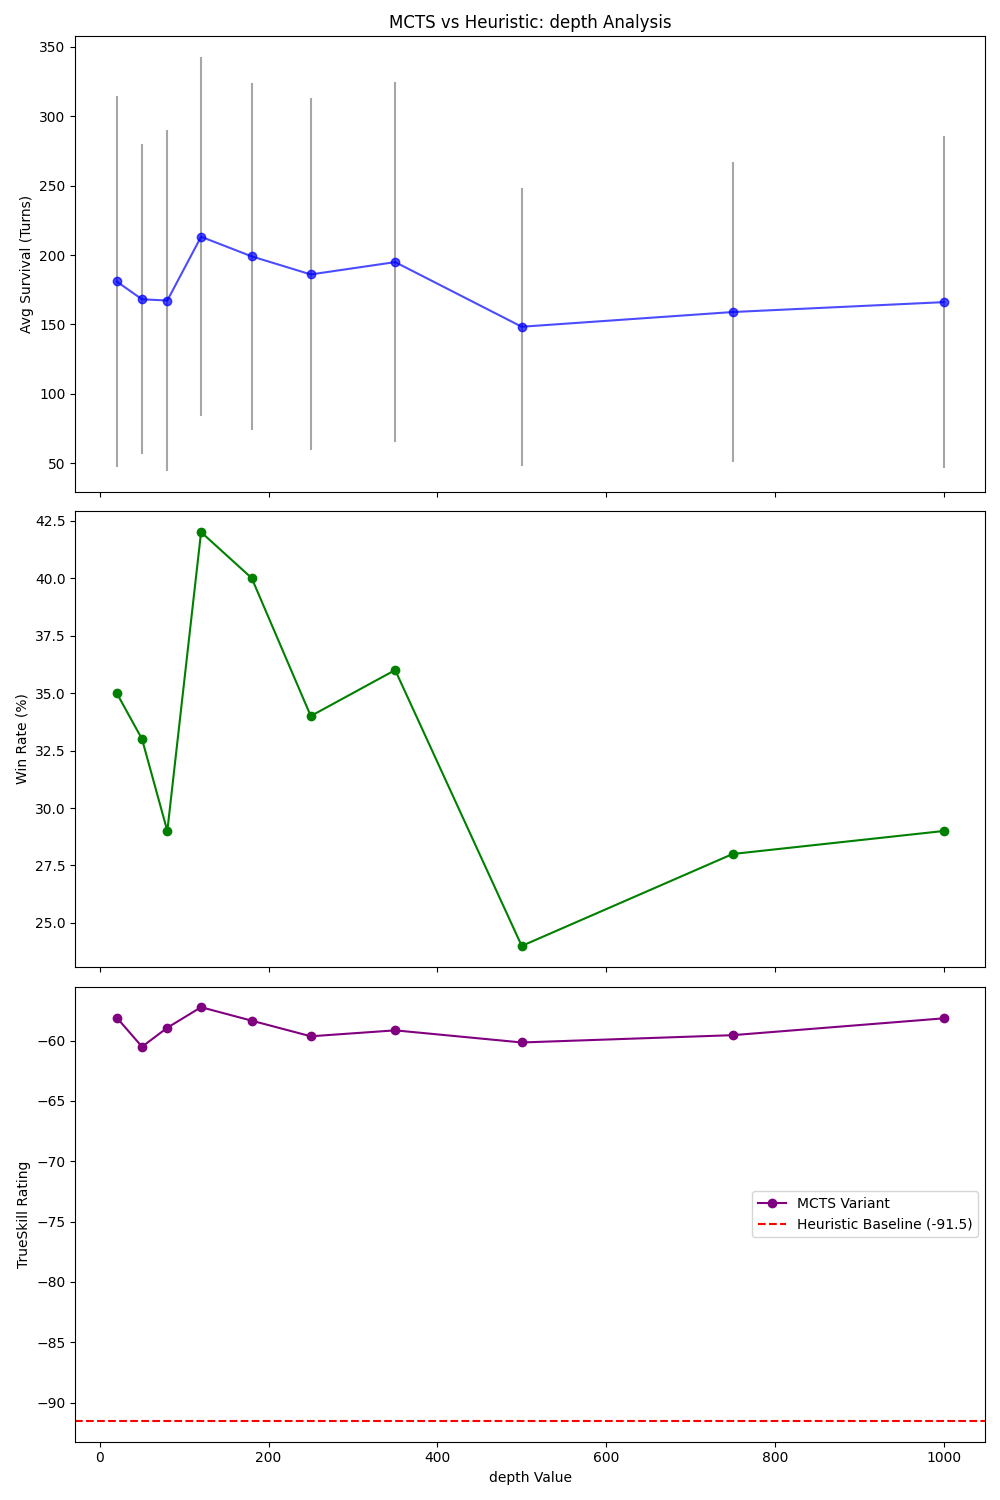
\includegraphics[width=\linewidth]{Figures/depth_metrics_plot_1000_games.png}
        \caption{Same as in \ref{fig:Cp} but now we explored a rollout depth ranging from 20 to 1000 steps at a fixed $C_p$ value (2.71). }
        \label{fig:sub2}
    \end{subfigure}
    
    \caption{Hyper-parameter exploration of the exploration constant and rollout depth in the MCTS agents. In total 1000 games were run consisting of one MCTS agent against 3 heuristics. In order to isolate the effect of the hyper-parameter we fixed the other parameter at a value. In the plots we present the average turns, win rates as well as TrueSkill ratings per hyper-parameter increment. In addition, we assign a heuristic baseline in the TrueSkill Rating as a reference point to our results.  }
    \label{fig:hyperparameter exploration}
\end{figure}



\section{Further improvements}
\subsection{Progressive Bias for heuristic action reduction}

In order to incorporate domain knowledge into the tree traversal, we further improve the MCTS stages by utilizing Progressive Bias. Contrary to the random rollouts, where the agent treats all moves with equal curiosity, this improvement aims for our agent to select promising moves based on simple heuristics, even before any rollouts have been performed for that node. Our implementation modifies the standard UCB formula to include this bias term. As we discussed in Section \ref{sec:heur-agent}, we calculate a reward when we expand a new node with out heuristic agent. Here, we utilize this reward as the bias component to guide our simulations. The bias becomes progressive as it is divided by the number of visits; when visit counts are low heuristics dominate the movement selection, but their influence is minor as the agent gathers information from the rollouts. Therefore, the selection of child nodes for expansion is done by maximizing the following formula:
\begin{equation}
    PB = UCB1 + \frac{\Delta \cdot P_b}{n_j+1}
\end{equation}
Where with $PB$ we assign the new selection function that incorporates Progressive Bias term in addition to the UCB1. In the bias term, we assign as $\Delta$ the reward calculation of the heuristic agent, $P_b$ is the weight of that bias. Through that weight we can influence the relationship between the heuristic and MCTS agent ensuring a value that maximizes the performance of our agents. This is an improvement of the heuristic rollout implementation we did before in our MCTS stages as we can now fine tune the dominance of the heuristics. 

Similarly to the hyper-parameter exploration we did in Section \ref{sec:hyperparameter-exploration}, we explore the effect of the weight $P_b$, by running a tournaments of 1000 games. The initial set up consists of one MCTS agent with a progressive bias implementation against 3 MCTS agents utilizing the standard UCB1 formula. At each game we varied the $P_b$ weight in a range of 0 to 150. We present the results in Figure \ref{fig:progressive-bias} for which we show the average turns, win rate and true skill rating per increment of $P_b$ weight. Given that the TrueSkill rating is the most accurate measure for the performance of our agents we find that we get the highest score for a $P_b$ weight of 3. 

\begin{figure}
    \centering
    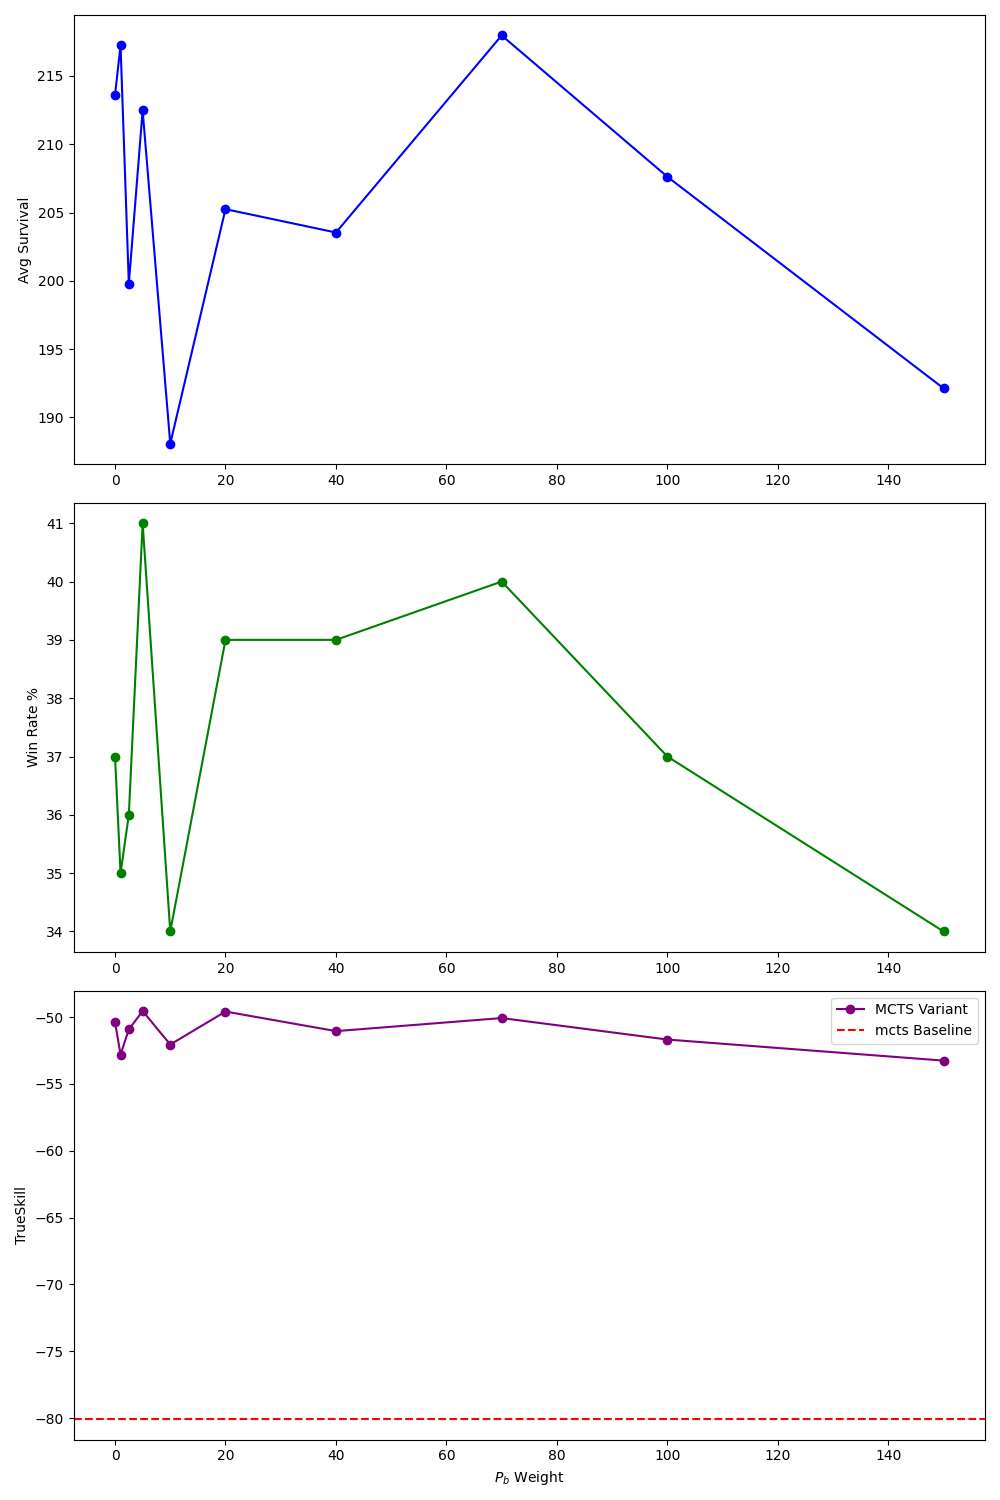
\includegraphics[width=0.5\linewidth]{Figures/pb_weight_vs_mcts_1000_games.png}
    \caption{Hyper-parameter exploration of the $P_b$ weight in the progressive bias implementation. In total 1000 games were run consisting of one MCTS agent with the improvement against 3 using the standard UCB1 formula for selection. In the plots we present the average turn, win rates as well as TrueSkill ratings per $P_b$ value. In addition, we assign a MCTS baseline in the TrueSkill Rating as a reference point to our results.  }
    \label{fig:progressive-bias}
\end{figure}

\subsection{Rapid Value Action Estimation in the selection}

Rapid Action Value Estimation (RAVE), also known as All Moves As First (AMAF) \citep{gelly2007combining}, addresses a fundamental sample-efficiency problem in MCTS. With a limited time budget, many tree nodes are visited only once or twice, making their UCB1 value estimates unreliable. The AMAF heuristic shares statistical information across the tree through the following intuition: \textit{if move $m$ led to a good outcome anywhere in the subtree below node $n$, then $m$ is probably also a good move at node $n$ itself.}

Each node stores two parallel sets of statistics: direct statistics $(v_n, N_n)$ for its own visits and cumulative reward, and AMAF statistics $(\tilde{v}_m, \tilde{N}_m)$ for every move $m$ observed anywhere in simulations passing through this node. The combined selection score is:
\begin{equation}
    Q_{\text{RAVE}}(n) = (1 - \beta)\,\frac{v_n}{N_n} + \beta\,\frac{\tilde{v}_m}{\tilde{N}_m}, \quad \beta = \sqrt{\frac{k}{3N_n + k}}
\end{equation}
with equivalence parameter $k=100$. The weight $\beta$ starts near 1 when a node is new (trusting AMAF statistics) and decays to 0 as direct evidence accumulates (trusting per-node statistics). The value $k=100$ places equal weight on both estimates when $N_n \approx 33$ visits, which matches the low-iteration regime of our 0.1-second time budget.

Unlike Progressive Bias, which modifies the expansion step with a fixed heuristic bias, RAVE updates dynamically using evidence collected during rollouts. This makes RAVE adaptive — as more simulations run, the AMAF estimates improve and the selection formula shifts weight accordingly. The two improvements are complementary: Progressive Bias focuses early exploration on promising branches, while RAVE refines selection estimates as the tree matures.

\pagebreak
\section{Results}\label{sec:results}
As we have discussed, we have implemented several agents used in modern games to win a battlesnake game. Our implementations include agents with two heuristic modes (competitive and friendly), MCTS with random and heuristic rollouts as well as two MCTS improvements with a progressive bias or RAVE in the selection phase. We first compare the two heuristic agents against the MCTS with random and heuristic rollouts. We perform a tournament of 1000 games for which we assigned the four different type of agents and recorded the true skill rating, win percentage as well as the average turn distribution per agent. In a similar manner, we performed the same tournament but now in the MCTS with the heuristic agent we implemented a progressive bias term with $P_b=3$. We present the results in Figure \ref{fig:tournaments}. Overall, we see that the MCTS agents outperform the heuristic ones with an overall higher TrueSkill score and win rate. Heuristic and random rollouts resulted in very similar performances in both the win rates and TrueSkill scores. The MCTS agent with the progressive bias implementation did not show any significant improvement relative to the random rollout, despite showing different behaviours during the game.

\subsection{RAVE and Paranoid Search Comparison}

To evaluate the RAVE improvement and the paranoid search agent, we ran an additional 16-game tournament on an 11$\times$11 board with all four implementations competing simultaneously: the greedy heuristic agent, vanilla MCTS with UCB1, MCTS augmented with RAVE and heuristic-biased expansion, and the paranoid search agent with alpha-beta pruning. Each agent was given a 0.1-second thinking budget per move. Agent ratings were computed using TrueSkill \citep{herbrich2006trueskill}; Table~\ref{tab:rave-results} shows the final leaderboard.

\begin{table}[H]
\centering
\caption{Tournament leaderboard — 16 games comparing RAVE and paranoid search against baselines}
\label{tab:rave-results}
\begin{tabular}{lrrrrc}
\hline
\textbf{Algorithm} & $\mu$ & $\sigma$ & \textbf{Conservative} ($\mu{-}3\sigma$) & \textbf{Wins} & \textbf{Avg.\ Turn} \\
\hline
MCTS + RAVE                   & 32.25 & 1.91 & \textbf{26.52} & 10 & 201.3 \\
Vanilla MCTS (UCB1)            & 30.94 & 1.98 & 25.01          &  5 & 134.0 \\
Paranoid Search (Alpha-Beta)   & 20.78 & 2.64 & 12.87          &  1 & 135.8 \\
Greedy Heuristic               & 14.61 & 3.99 &  2.64          &  0 &  64.0 \\
\hline
\end{tabular}
\end{table}


\begin{figure}[h]
    \centering
    
    \begin{subfigure}{0.49\textwidth}
        \centering
        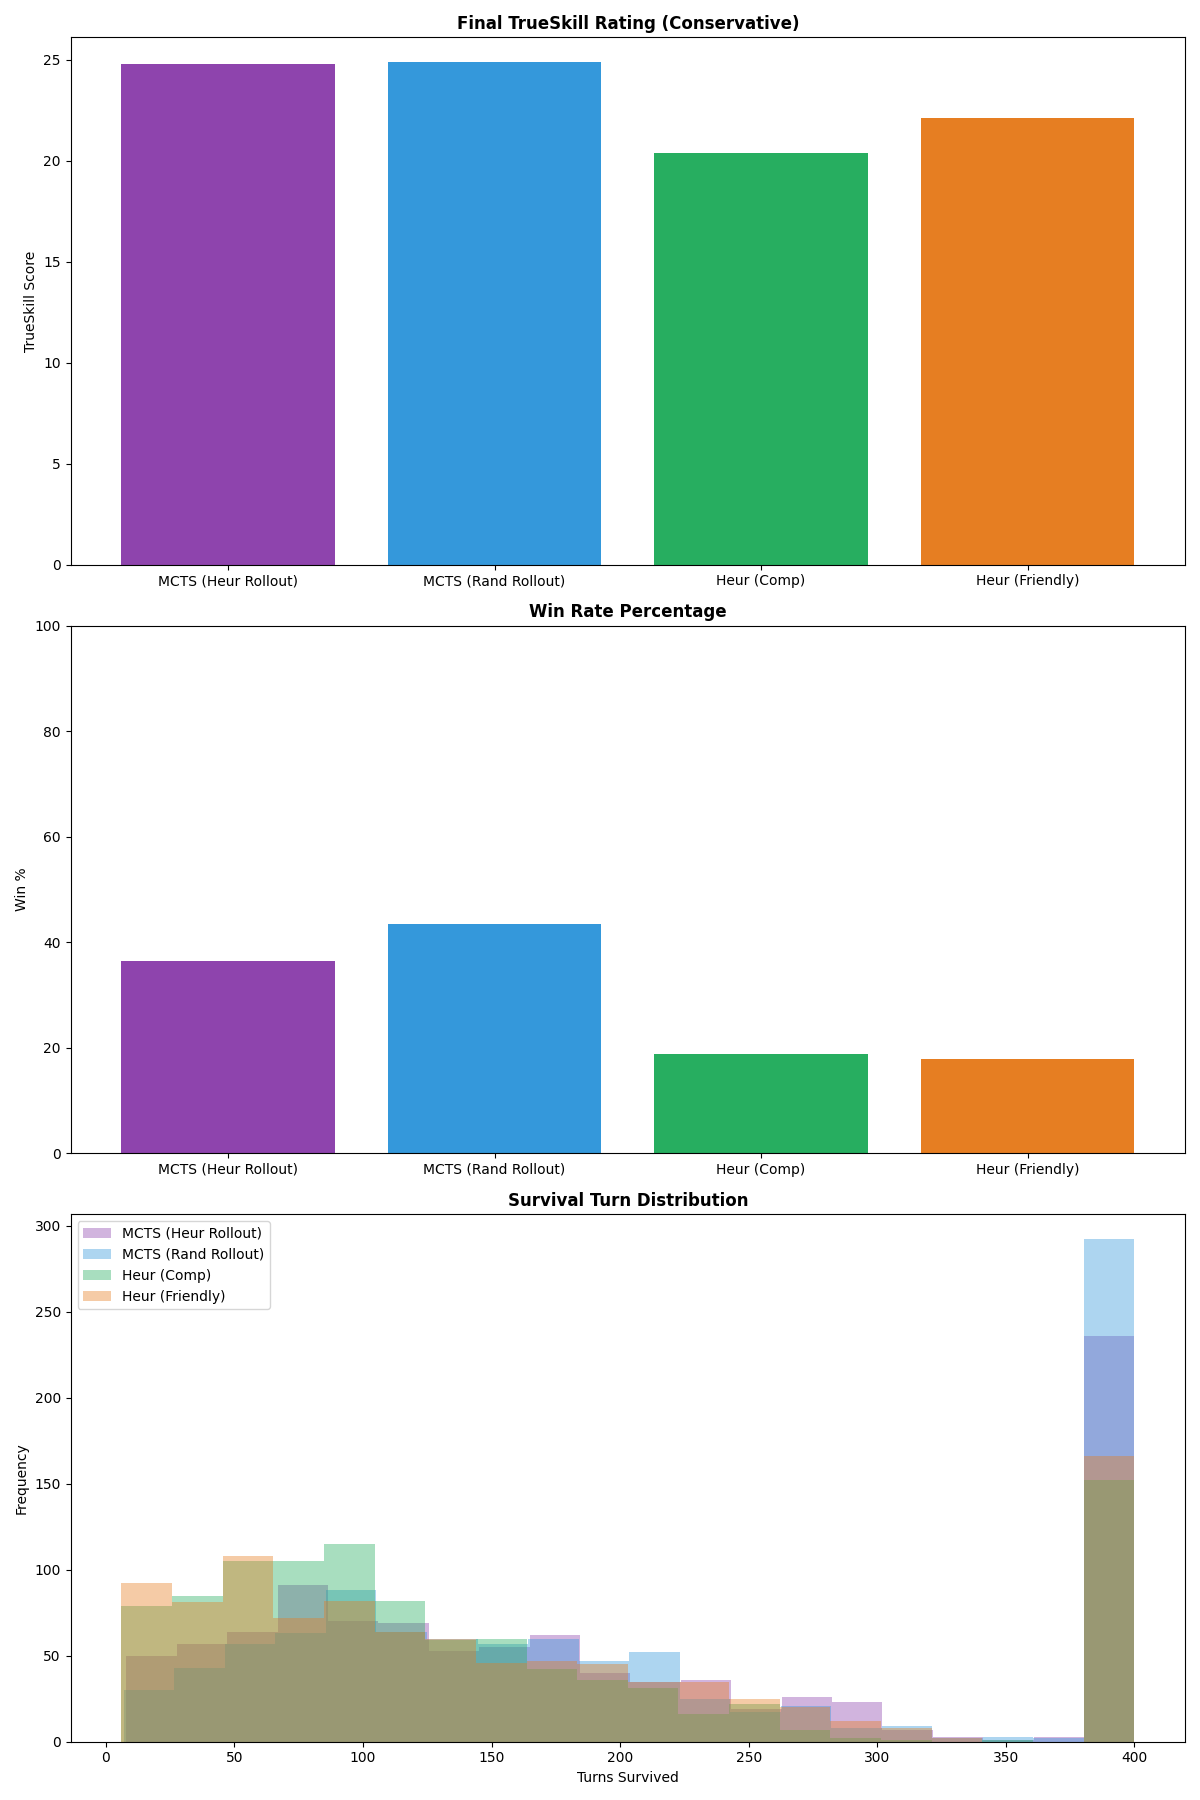
\includegraphics[width=\linewidth]{Figures/melee_comprehensive_1000_games.png}
        \caption{ Tournament of two heuristic agents (friendly and competitive modes) against two MCTS (random and heuristic rollout).}
        \label{fig:tourn1}
    \end{subfigure}
    \hfill
    \begin{subfigure}{0.49\textwidth}
        \centering
        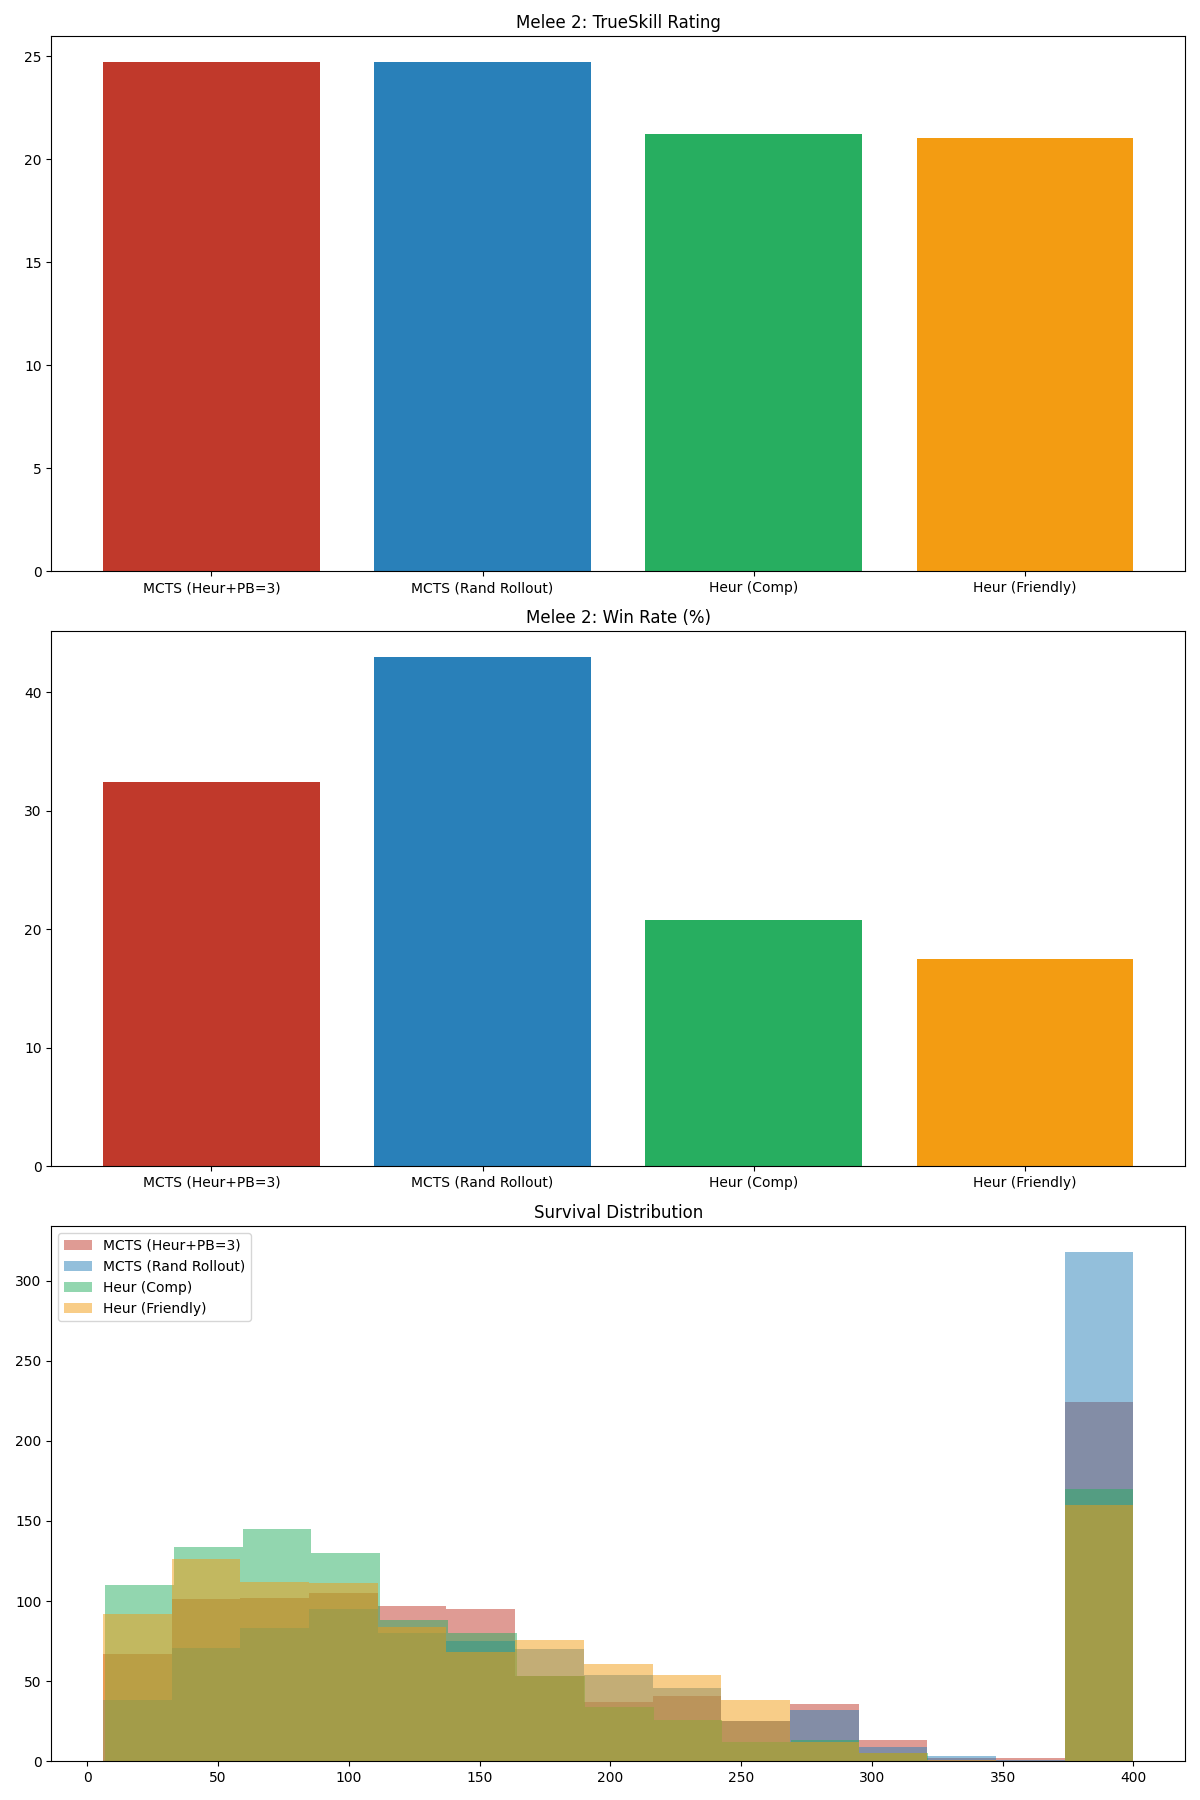
\includegraphics[width=\linewidth]{Figures/melee2_stats_1000_games.png}
        \caption{Same as in \ref{fig:tourn1} only the MCTS with the heuristic rollout includes the progressive bias improvement with $P_b = 3$). }
    \end{subfigure}
    
    \caption{Comparison of the agent's performances. In total, 1000 games were performed and in the plots we present the TrueSkill ratings, win rates as well as the survival turn distribution per agent. }
    \label{fig:tournaments}
\end{figure}




\section{Discussion}\label{sec:discussion}

\subsection{RAVE Improves Over Vanilla MCTS}

The tournament results in Table~\ref{tab:rave-results} confirm that MCTS + RAVE outperforms vanilla MCTS, winning 10 out of 16 games (62.5\%) compared to 5 wins (31.25\%) for vanilla UCB1. The conservative TrueSkill score of 26.52 versus 25.01 represents a meaningful gap given the 16-game sample. The RAVE agent also survived significantly longer on average (201.3 turns versus 134.0), indicating that RAVE's adaptive value estimates produce more consistent, safer play rather than occasional wins by chance. This confirms the core motivation for RAVE: bootstrapping value estimates from all simulations below a node is particularly valuable when the per-node visit counts are low, which is exactly the regime imposed by our 0.1-second time budget.

\subsection{Paranoid Search Underperformed Expectations}

The paranoid search agent achieved only 1 win (6.25\%) and a conservative score of 12.87, placing closer to the greedy heuristic than to the MCTS variants. This outcome is worth examining carefully. The paranoid assumption — that all opponents act as a perfectly coordinated coalition to eliminate us — leads to a strongly defensive playing style. While theoretically sound as a worst-case bound \citep{sturtevant2006effective}, this conservatism is often misaligned with actual opponent behaviour in BattleSnakes, where three independent agents each pursue their own survival rather than coordinating against a single target. The result is that the paranoid agent avoids many moves that are in fact safe, restricting itself to a narrow set of options and sacrificing positional advantage.

Additionally, the quality of the leaf evaluation function limits how deep the search can meaningfully reason. At depth 2–3, the heuristic evaluation captures spatial availability and food proximity but cannot model the medium-term consequences of being cornered or cut off. MCTS compensates for this through rollouts that propagate terminal outcomes, while paranoid search relies entirely on the quality of the static evaluator at leaf nodes.

\subsection{Consistent Two-Tier Structure}

Across both the 1000-game tournament (Figure~\ref{fig:tournaments}) and the 16-game comparison (Table~\ref{tab:rave-results}), the same two-tier structure emerges: MCTS-based agents win the overwhelming majority of games, while the greedy heuristic agent wins almost none. This robustly confirms that look-ahead search — regardless of the specific variant — provides a decisive advantage over greedy single-step evaluation in 4-player BattleSnakes.

\section{Future Work}\label{sec:future work}

The current RAVE implementation, while effective, represents only one of several established directions for improving Monte Carlo Tree Search. A natural next step is to explore alternative value-sharing schemes.

\textbf{GRAVE (Generalised RAVE)} \citep{cazenave2015generalized} extends the AMAF concept by sharing statistics across multiple ancestor nodes rather than just within each node's subtree. In low-iteration regimes, GRAVE produces more stable value estimates than standard RAVE, since it draws on a larger pool of simulation data. Given that our agents complete only 30–50 iterations per 0.1-second move, GRAVE would likely offer further gains.

\textbf{PUCT and neural-guided search}, as used in AlphaZero \citep{silver2017mastering}, replace the UCB1 exploration bonus with a learned prior probability over moves. Rather than relying on AMAF statistics or a hand-crafted heuristic, a small policy network trained via self-play could guide both expansion and rollouts. Even a shallow network trained on game outcomes could substantially reduce rollout variance compared to the current heuristic policy.

\textbf{Soft opponent modelling} offers an alternative to the paranoid assumption. Rather than treating all opponents as a perfectly coordinated adversary, a Bayesian opponent model \citep{albrecht2018autonomous} maintains a distribution over plausible opponent policies and weights rollout outcomes accordingly. This strikes a balance between the overly conservative paranoid approach and the overly optimistic assumption of random opponent play, and has been shown to improve performance in repeated multi-agent games.

\textbf{Progressive widening} \citep{coulom2007computing} addresses the large branching factor of BattleSnakes by limiting the number of children expanded at each node as a function of visit count. This concentrates early rollouts on the most promising moves and avoids the diffusion of statistics across rarely-visited branches, which is especially relevant for a 4-player game where the joint action space grows as $4^4 = 256$ per turn.

\textbf{Systematic hyperparameter tuning} for the RAVE equivalence parameter $k$ and the MCTS exploration constant $C_p$ using population-based training \citep{jaderberg2017population} could provide further gains. The optimal values for these parameters in a 4-player, stochastic game with hazard mechanics may differ considerably from the theoretical defaults derived for 2-player zero-sum games.

\section{Conclusions}\label{sec:conclusion}

We built and evaluated four BattleSnake agents of increasing sophistication: a greedy heuristic agent, vanilla MCTS with UCB1, MCTS augmented with RAVE and heuristic-biased expansion, and a paranoid search agent with alpha-beta pruning.

The principal finding across both 1000-game and 16-game tournaments is that look-ahead search strongly dominates greedy evaluation. The MCTS agents collectively won over 90\% of games against heuristic-only opponents. Among search agents, MCTS + RAVE achieved the best performance, winning 62.5\% of games in the 16-game comparison and consistently outsurviving vanilla MCTS. The RAVE improvement proves particularly effective in the low-iteration regime imposed by the 0.1-second time budget, where bootstrapping value estimates from sibling simulations compensates for sparse per-node visit counts.

The paranoid search agent, despite its theoretical guarantees, underperformed MCTS in practice due to the over-conservative paranoid assumption and the limited expressiveness of the static leaf evaluator. This highlights an important insight: in stochastic multi-player games where opponents are not coordinating, worst-case adversarial search is not always the best model.

Future work should focus on learned value functions to replace hand-crafted evaluation, generalised RAVE for better sample efficiency, and soft opponent models that better reflect actual multi-agent dynamics.

\bibliographystyle{apalike}
\bibliography{bib}

\end{document}